\section{Model Structure \& Notation}\label{model.str}
The model aims to capture heterosexual HIV transmission among the Swati population aged 15--49.
The model stratifies the modelled population along five dimensions, including:
2 sexes~($s$), 4 activity groups~($i$), 6 HIV states~($h$), and 5 cascade states~($c$);
the fifth dimension tracks seroconcordant \hivp partnerships
and includes strata for each of 4 partnership types ($p$) plus 1 extra stratum
--- see \sref{foi.prop} for full details.
In total, $2 \times 4 \times (1 + 5 \times 5 \times 5) = 1008$ states are modelled,
since the cascade and partnership dimensions are only applicable to PLHIV ($h>1$).
These dimensions are summarized in Table~\ref{tab:model.dims} and Figure~\ref{fig:model}.
Two types of sex acts ($a$) are also considered.
\begin{table}
  \centering
  \caption{Overview of model dimensions and stratifications}
  \label{tab:model.dims}
  \begin{tabular}{lccl}
  \toprule
  Dimension                  & \multicolumn{2}{c}{Index} & Strata \\
  \midrule
  \textbf{Sex}               & ($s$) & 1 & Heterosexual Women    \\
                             &       & 2 & Heterosexual Men      \\[1ex]
  \textbf{Activity group}    & ($i$) & 1 & Lowest Activity       \\
                             &       & 2 & Medium Activity       \\
                             &       & 3 & Lower Risk Sex Work   \\
                             &       & 4 & Higher Risk Sex Work  \\[1ex]
  \textbf{HIV status}        & ($h$) & 1 & Susceptible           \\
                             &       & 2 & Acute HIV             \\
                             &       & 3 & CD4 $>$ 500           \\
                             &       & 4 & 350 $<$ CD4 $<$ 500   \\
                             &       & 5 & 200 $<$ CD4 $<$ 350   \\
                             &       & 6 & CD4 $<$ 200 (AIDS)    \\[1ex]
  \textbf{ART cascade}       & ($c$) & 1 & Undiagnosed           \\
                             &       & 2 & Diagnosed             \\
                             &       & 3 & On ART                \\
                             &       & 4 & Virally Suppressed    \\
                             &       & 5 & Unlinked from Care    \\[1ex] % TODO: implement this change in code
  \textbf{Partnership types} & ($p$) & 1 & Main / Spousal        \\
                             &       & 2 & Casual                \\
                             &       & 3 & Occasional Sex Work   \\
                             &       & 4 & Regular Sex Work      \\[1ex]
  \textbf{Sex act types}     & ($a$) & 1 & Vaginal               \\
                             &       & 2 & Anal                  \\
  \bottomrule
\end{tabular}
  \floatfoot{\centering See footnote \ref{foot:code.note} regarding indices in the code.}
\end{table}
\par
Sexual activity groups were defined to reflect common stratifications in the available data,
and persistent differences in HIV incidence and prevalence
\cite{SDHS2006,Bicego2013,Justman2016,SHIMS2}
--- reflecting acquisition and/or onward transmission risk.
The lowest sexual activity group ($i=1$) comprises
individuals who had 0-1 sexual partners in the past 12 months (p12m),
but did not engage in sex work.
The medium activity group ($i=2$) similarly comprises
individuals who had 2+ sexual partners in p12m
but did not engage in formal sex work.
The highest two activity groups among women ($i=3,4$) comprise
lower and higher risk FSW (see \sref{model.par.fsw} for more details), and
the highest two activity groups among men ($i=3,4$) likewise comprise
lower and higher risk clients of FSW.
% TODO: (?) Watts2010 re pimps, etc.
\par
Four types of sexual partnerships are modelled,
in order to capture different partnership durations relevant to Chapter~\ref{foi},
and different trends in condom use relevant to inferred transmission dynamics across groups
--- \ie all downstream analyses.
The four partnership types are:
long-term/spousal partnerships ($p=1$, lowest condom use, 14--19 years);
short-term partnerships ($p=2$, medium condom use, 3--18 months);
one-off new/occasional sex work partnerships ($p=3$, highest condom use, 1 sex act);
and regular sex work partnerships ($p=4$, medium condom use, 2--24 months).
Figure~\ref{fig:model.risk} illustrates
the modelled activity groups and possible partnership types between them.
\begin{figure}
  \begin{subfigure}{\linewidth}
    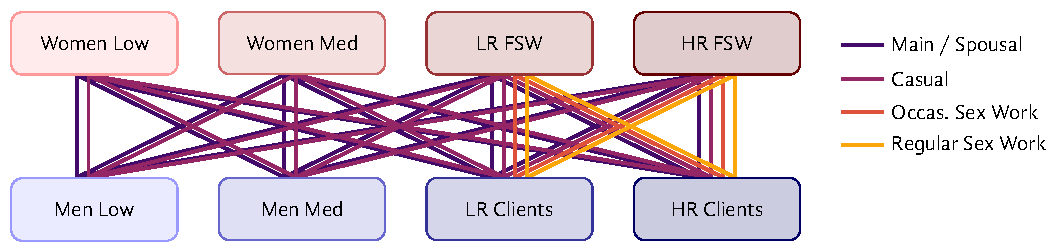
\includegraphics[scale=.8]{model.risk}
    \caption{Activity groups and partnership types}
    \label{fig:model.risk}
  \end{subfigure}
  \begin{subfigure}{\linewidth}
    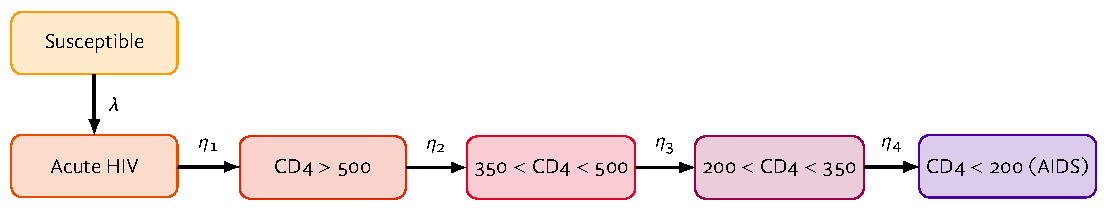
\includegraphics[scale=.8]{model.hiv}
    \caption{HIV states}
    \label{fig:model.hiv}
  \end{subfigure}
  \begin{subfigure}{\linewidth}
    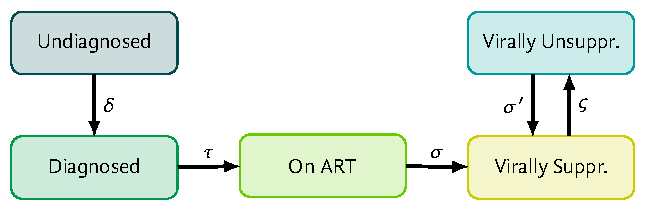
\includegraphics[scale=.8]{model.cascade}
    \caption{ART cascade states}
    \label{fig:model.cascade}
  \end{subfigure}
  \caption{Model structure and transitions}
  \label{fig:model}
  \floatfoot{\ffpops;
    CD4: CD4+ T-cell count per mm\tsup{3};
    Not shown: turnover amongst activity groups in \sfref{fig:model.risk}.}
\end{figure}
\par
HIV infection is stratified into
acute-HIV and stages defined by CD4 count (Figure~\ref{fig:model.hiv})
to reflect changes in mortality~\cite{Mangal2017},
historical ART eligibility~\cite{EswMOH2006,EswMOH2010,EswMOH2015,EswMOH2018},
and, with CD4 as a proxy for viral load, infectiousness~\cite{Boily2009}.
The modelled ART cascade (Figure~\ref{fig:model.cascade})
includes the steps associated with the ``90-90-90'' targets,
plus a generic ``virally un-suppressed'' state reflecting any combination of
treatment failure, discontinuation, or loss to follow-up after achieving viral suppression.
Loss to follow-up prior to viral suppression is not explicitly modelled,
but subsumed into rates of ART initiation and viral suppression.
%---------------------------------------------------------------------------------------------------
\paragraph{Notation}
If $X$ is a variable (\eg population, parameter, calibration target)
stratified by dimensions $a,b,c$,
then $X_{ab_{1}c_{23}}$ denotes the values of $X$ for
a particular but \emph{unspecified} stratum of $a$,
the \emph{specific} stratum $b = 1$,
and the \emph{aggregated} strata $c = 2,3$
(the aggregating operation is context-dependent, \eg sum for probabilities).
Additionally, the indices $sihc$ from Table~\ref{tab:model.dims} denote ``self'' strata,
whereas $s'i'h'c'$ denote ``other'' strata --- \ie individuals' partners.%
\footnote{\label{foot:code.note}%
  In the code: R uses one-based indexing, which match the notation here directly,
  while Python uses zero-based indexing, which therefore appear as $i \rightarrow i-1$ in the code.
  Also, the model code reorders states in the ART Cascade dimension for computational efficiency,
  with $c={}$1:~Undiagnosed; 2:~Diagnosed; 3:~Virally~Un-suppressed; 4:~On~ART; 5:~Virally~Suppressed.}
Finally, I re-use several dummy variables throughout the chapter:
$\rho$ for proportions, $\lambda$ for rates, $T$ for time periods, and $f$ for constants.
